\chapter{Python}
\begin{center}
  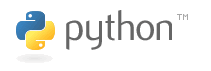
\includegraphics[width=140px]{img/python.png} \\
  \textbf{\url{http://python.org}}
\end{center}
\begin{quote}
  \textit{Python is a programming language that lets you work more quickly and integrate your systems more effectively.
          You can learn to use Python and see almost immediate gains in productivity and lower maintenance costs.}
\end{quote}

\section{IPython}
Python selbst kommt mit einer interaktiven Kommandozeile (genauer: einer REPL\footnote{read–eval–print loop}-Umgebung).
Um einen Einblick in die Sprache zu erhalten, ist diese eigentlich vollkommen ausreichend.
Sie bietet die Möglichkeit, interaktiv mit der Sprache in Kontakt zu kommen.
IPython erlaubt zusätzlich, auf die Shell zuzugreifen und interaktive Sitzungen zu speichern.
Gestartet wird IPython auf der Kommandozeile mit
\begin{verbatim}
ipython3
\end{verbatim}
und meldet sich (zum Beispiel hier unter OS X mit Python 3.2.3) mit der Ausgabe
\begin{verbatim}
Python 3.2.3 (default, Apr 13 2012, 00:15:25) 
Type "copyright", "credits" or "license" for more information.

IPython 0.13 -- An enhanced Interactive Python.
?         -> Introduction and overview of IPython's features.
%quickref -> Quick reference.
help      -> Python's own help system.
object?   -> Details about 'object', use 'object??' for extra details.

In [1]: 
\end{verbatim}
Um IPython zu beenden gibt es die Befehle \texttt{exit}, \texttt{exit()}, \texttt{quit}, \texttt{quit()} und natürlich \texttt{Ctrl-D}.

\section{Syntax}
Grundsätzlich ist die Python-Syntax sehr einfach und intuitiv.
In vielen Punkten erinnert sie eher an eine Scriptsprache.
In einer interaktiven Sitzung (z.B. IPython) können zum Einstieg einfache mathematische Berechnungen durchgeführt werden:
\begin{verbatim}
In [1]: 1 + 2
Out[1]: 3

In [2]: 1 * 2
Out[2]: 2
\end{verbatim}

\subsection{Variablen}
Natürlich gibt es Variablen. Ihre Verwendung ist denkbar einfach:
\begin{verbatim}
In [3]: a = 2

In [4]: a
Out[4]: 2

In [5]: b = 1 + 1

In [6]: b
Out[6]: 2
\end{verbatim}
Variablennamen können Buchstaben, Zahlen und Unterstrichte enthalten, dürfen jedoch nicht mit einer Ziffer beginnen.

\subsection{Operatoren}
Wie aus dem obigen Beispiel hervorgeht, gibt es in Python \textbf{mathematische Operatoren}.
In \autoref{tab:op_mat} sind diese dargestellt.

\begin{table}[H]
  \centering{}
  \caption{Mathematische Operatoren}
  \label{tab:op_mat}
  \begin{tabular}{c l c c}
    \toprule
    Op.         & Funktion         & Beispiel         & Ergebnis \\
    \midrule
    \texttt{+}  & Addition         & \texttt{1 + 2}   & \texttt{3} \\
    \texttt{-}  & Subtraktion      & \texttt{1 - 2}   & \texttt{-1} \\
    \texttt{*}  & Multiplikation   & \texttt{1 * 2}   & \texttt{2} \\
    \texttt{/}  & Division         & \texttt{1 / 2}   & \texttt{0.5} \\
    \texttt{\%} & Modulo           & \texttt{11 \% 2} & \texttt{1} \\
    \texttt{**} & Exponent         & \texttt{2**3}  & \texttt{8} \\
    \texttt{//} & Ganzzahldivision & \texttt{5 // 2}  & \texttt{2} \\
    \bottomrule
  \end{tabular}
\end{table}

\textbf{Zuweisungsoperatoren} setzen sich aus einem mathematischen Operator und einem Gleichheitszeichen zusammen.
Mit ihnen kann gleichzeitig eine Berechnung und eine Zuweisung durchgeführt werden, zum Beispiel:
\begin{verbatim}
In [7]: a = 2

In [7]: a *= 3

In [8]: a
Out[8]: 6
\end{verbatim}

Mit Hilfe von \textbf{Vergleichsoperatoren} (siehe \autoref{tab:op_comp}) lassen sich Vergleiche durchführen.
\begin{table}[H]
  \centering{}
  \caption{Vergleichsoperatoren}
  \label{tab:op_comp}
  \begin{tabular}{c l c c}
    \toprule
    Op.             & Funktion            & Beispiel        & Ergebnis \\
    \midrule
    \texttt{==}     & Gleich              & \texttt{1 == 1} & \texttt{True} \\
    \texttt{!=}     & Ungleich            & \texttt{2 != 1} & \texttt{True} \\
    \texttt{>}      & Größer              & \texttt{2 > 1}  & \texttt{True} \\
    \texttt{<}      & Kleiner             & \texttt{1 < 2}  & \texttt{True} \\
    \texttt{>=}     & Größer oder gleich  & \texttt{2 >= 1} & \texttt{True} \\
    \texttt{<=}     & Kleiner oder gleich & \texttt{1 <= 2} & \texttt{True} \\
    \bottomrule
  \end{tabular}
\end{table}

\subsection{Dateien}
 
python
    open
    file
        write
    range
    len
    string
        format
        join
    list
        append
        index
    dict
    sorted
    decimal
    math
        floor
        ceil
    convert
        str
        int
        float

\section{Bibliotheken}
\subsection{NumPy}
NumPy ist eine Bibliothek für Python, die diverse Features unterstützt, die wissenschaftliches Arbeiten deutlich erleichtern.
Einige davon sind
\begin{itemize}
  \item ein $n$-dimensionales Array-Objekt
  \item ausgeklügelte, durchdachte Funktionen für Optimierung, Integration und Interpolation
  \item die Möglichkeit C/C++- und Fortran-Code zu integrieren
  \item Tools für Lineare Algebra, Fouriertransformation, Statistik
  \item beliebige eigene Datentypen können definiert werden
\end{itemize}

\subsection{SciPy}
SciPy ist, ähnlich wie NumPy, eine Bibliothek, die wissenschaftliches Arbeiten erleichtert.
Insbesondere sind in dem Paket verschiedene Konstanten gespeichert, die im Praktikum oft gebraucht werden.
SciPy ist eine Erweiterung von NumPy, die vor allem vom NumPy-Array profitiert.
Es besitzt ebenfalls viele benutzerfreundliche und effiziente numerische Algorithmen für Integration und Optimierung.

\subsection{matplotlib}
Bei matplotlib handelt es ich um eine Bibliothek für Plots.
\begin{quote}
  \textit{matplotlib tries to make easy things easy and hard things possible.}
\end{quote}
Es dient dazu Plots, auch polare, sowie Fehlerbalken und noch vieles mehr zu Plotten.
Es bietet sehr viele Einstellungsmöglichkeiten mit denen man den Plot anpassen kann.
matplotlib bietet eine objektorientierte API, die erlaubt die Plots in Anwendungen einzubetten die generische GUI-Toolkits wie Qt oder GTK benutzen.
Es gibt ebenfalls PyLab, das die verwendung in IPython erleichtert.

\subsubsection{Objektorientiertes Interface}
\begin{figure}
  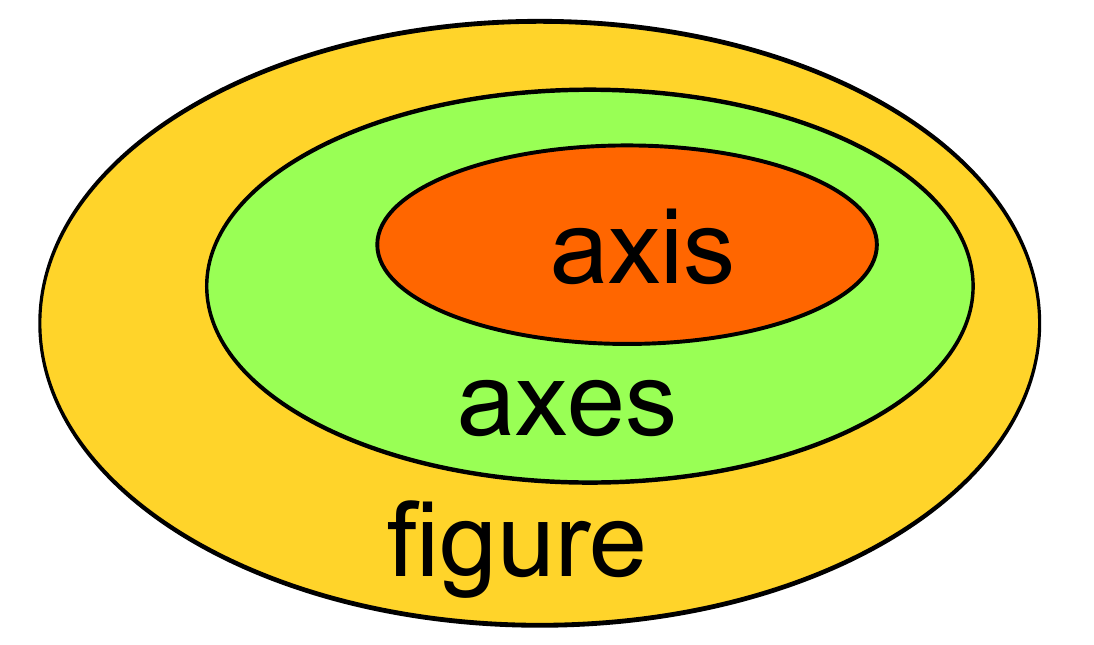
\includegraphics[width=150px]{img/matplotlib_v.png}
\end{figure}
\begin{itemize}
  \item figure: Leinwand, auf die Plots projiziert werden
  \item axes: enthält Plot, der beliebig in der figure plaziert werden kann
  \item axis: Koordinatenachsen 
\end{itemize}

\section{Python 2}
Falls man Python 2 verwendet, sollte jede \texttt{.py}-Datei so anfangen:
\begin{verbatim}
# coding=utf-8
from __future__ import division, print_function, unicode_literals
\end{verbatim}
Dann funktionieren Division, \texttt{print} und Unicode wie in Python 3.
Man sollte dann auch immer \texttt{python2} und \texttt{ipython2} aufrufen.

\section{Weiterführende Links}
\begin{itemize}
  \item Learn Python The Hard Way (Python 2): \url{http://learnpythonthehardway.org/}
  \item Dive Into Python 3: \url{http://www.diveintopython3.net/}
  \item Python v3 documentation: \url{http://docs.python.org/py3k/}
  \item PEP 8 -- Style Guide for Python Code: \url{http://www.python.org/dev/peps/pep-0008/}
  \item Tentative NumPy Tutorial: \url{http://www.scipy.org/Tentative\_NumPy\_Tutorial}
  \item NumPy and SciPy Documentation: \url{http://docs.scipy.org/doc/}
  \item matplotlib Documentation: \url{http://matplotlib.org/1.2.0/contents.html}
  \item matplotlib Gallery: \url{http://matplotlib.org/1.2.0/gallery.html}
  \item Python Uncertainties package: \url{http://packages.python.org/uncertainties/}
  \item SymPy: \url{http://sympy.org/en/index.html}
  \item matplotlib tutorial: \url{http://www.loria.fr/~rougier/teaching/matplotlib/}
  \item Python Scientific Lecture Notes: \url{http://scipy-lectures.github.com/}
  \item PyCon 2012: \url{http://pyvideo.org/category/17/pycon-us-2012}
    \begin{itemize}
      \item Plotting with matplotlib: \url{http://pyvideo.org/video/617/plotting-with-matplotlib}
      \item IPython: Python at your fingertips: \url{http://pyvideo.org/video/640/ipython-python-at-your-fingertips}
      \item IPython in-depth: high-productivity interactive and parallel python: \url{http://pyvideo.org/video/605/ipython-in-depth-high-productivity-interactive-a}
      \item Python for data lovers: explore it, analyze it, map it: \url{http://pyvideo.org/video/676/python-for-data-lovers-explore-it-analyze-it-m}
      \item Sage: Open Source Math in Python: \url{http://pyvideo.org/video/652/sage-open-source-math-in-python}
    \end{itemize}
  \item SciPy 2012: \url{http://pyvideo.org/category/20/scipy\_2012}
    \begin{itemize}
      \item Introduction to NumPy and matplotlib: \url{http://pyvideo.org/video/1190/introduction-to-numpy-and-matplotlib}
      \item Advanced matplotlib: \url{http://pyvideo.org/video/1344/advanced-matplotlib}
      \item IPython: tools for the entire lifecycle of research computing: \url{http://pyvideo.org/video/1221/ipython-tools-for-the-entire-lifecycle-of-resear}
      \item A tale of four libraries: \url{http://pyvideo.org/video/1211/a-tale-of-four-libraries}
    \end{itemize}
  \item SciPy 2011: \url{http://archive.org/search.php?query=subject\%3A\%22SciPy2011\%22}
\end{itemize}
